In this section the original operations of the mor1kx, concerning the write policy of the data cache, are briefly described to better understand which Verilog modules need to be modified and why.

\section{Write Through Implementation}
The followings are the relevant features offered before the changeover:
\begin{itemize}
	\item \textbf{\textit{write-through} write policy:} when a write occurs, data is written both to data cache and main memory;
	\item \textbf{no-write allocate:} on a write miss, data is directly written in main memory bypassing the data cache;
	\item \textbf{store buffer:} if enabled, during a store operation data is not only sent to the data cache, but also to the store buffer (a.k.a. write buffer). It is useful because bursts of writes are common. Moreover, it might prevent the processor from stalling.
\end{itemize}

The flow diagram in Figure \ref{wt_flow_diagram} depicts the series of procedures accomplished by the original implementation of the processor during read and write operations.

\begin{figure}[H]
	\begin{center}
		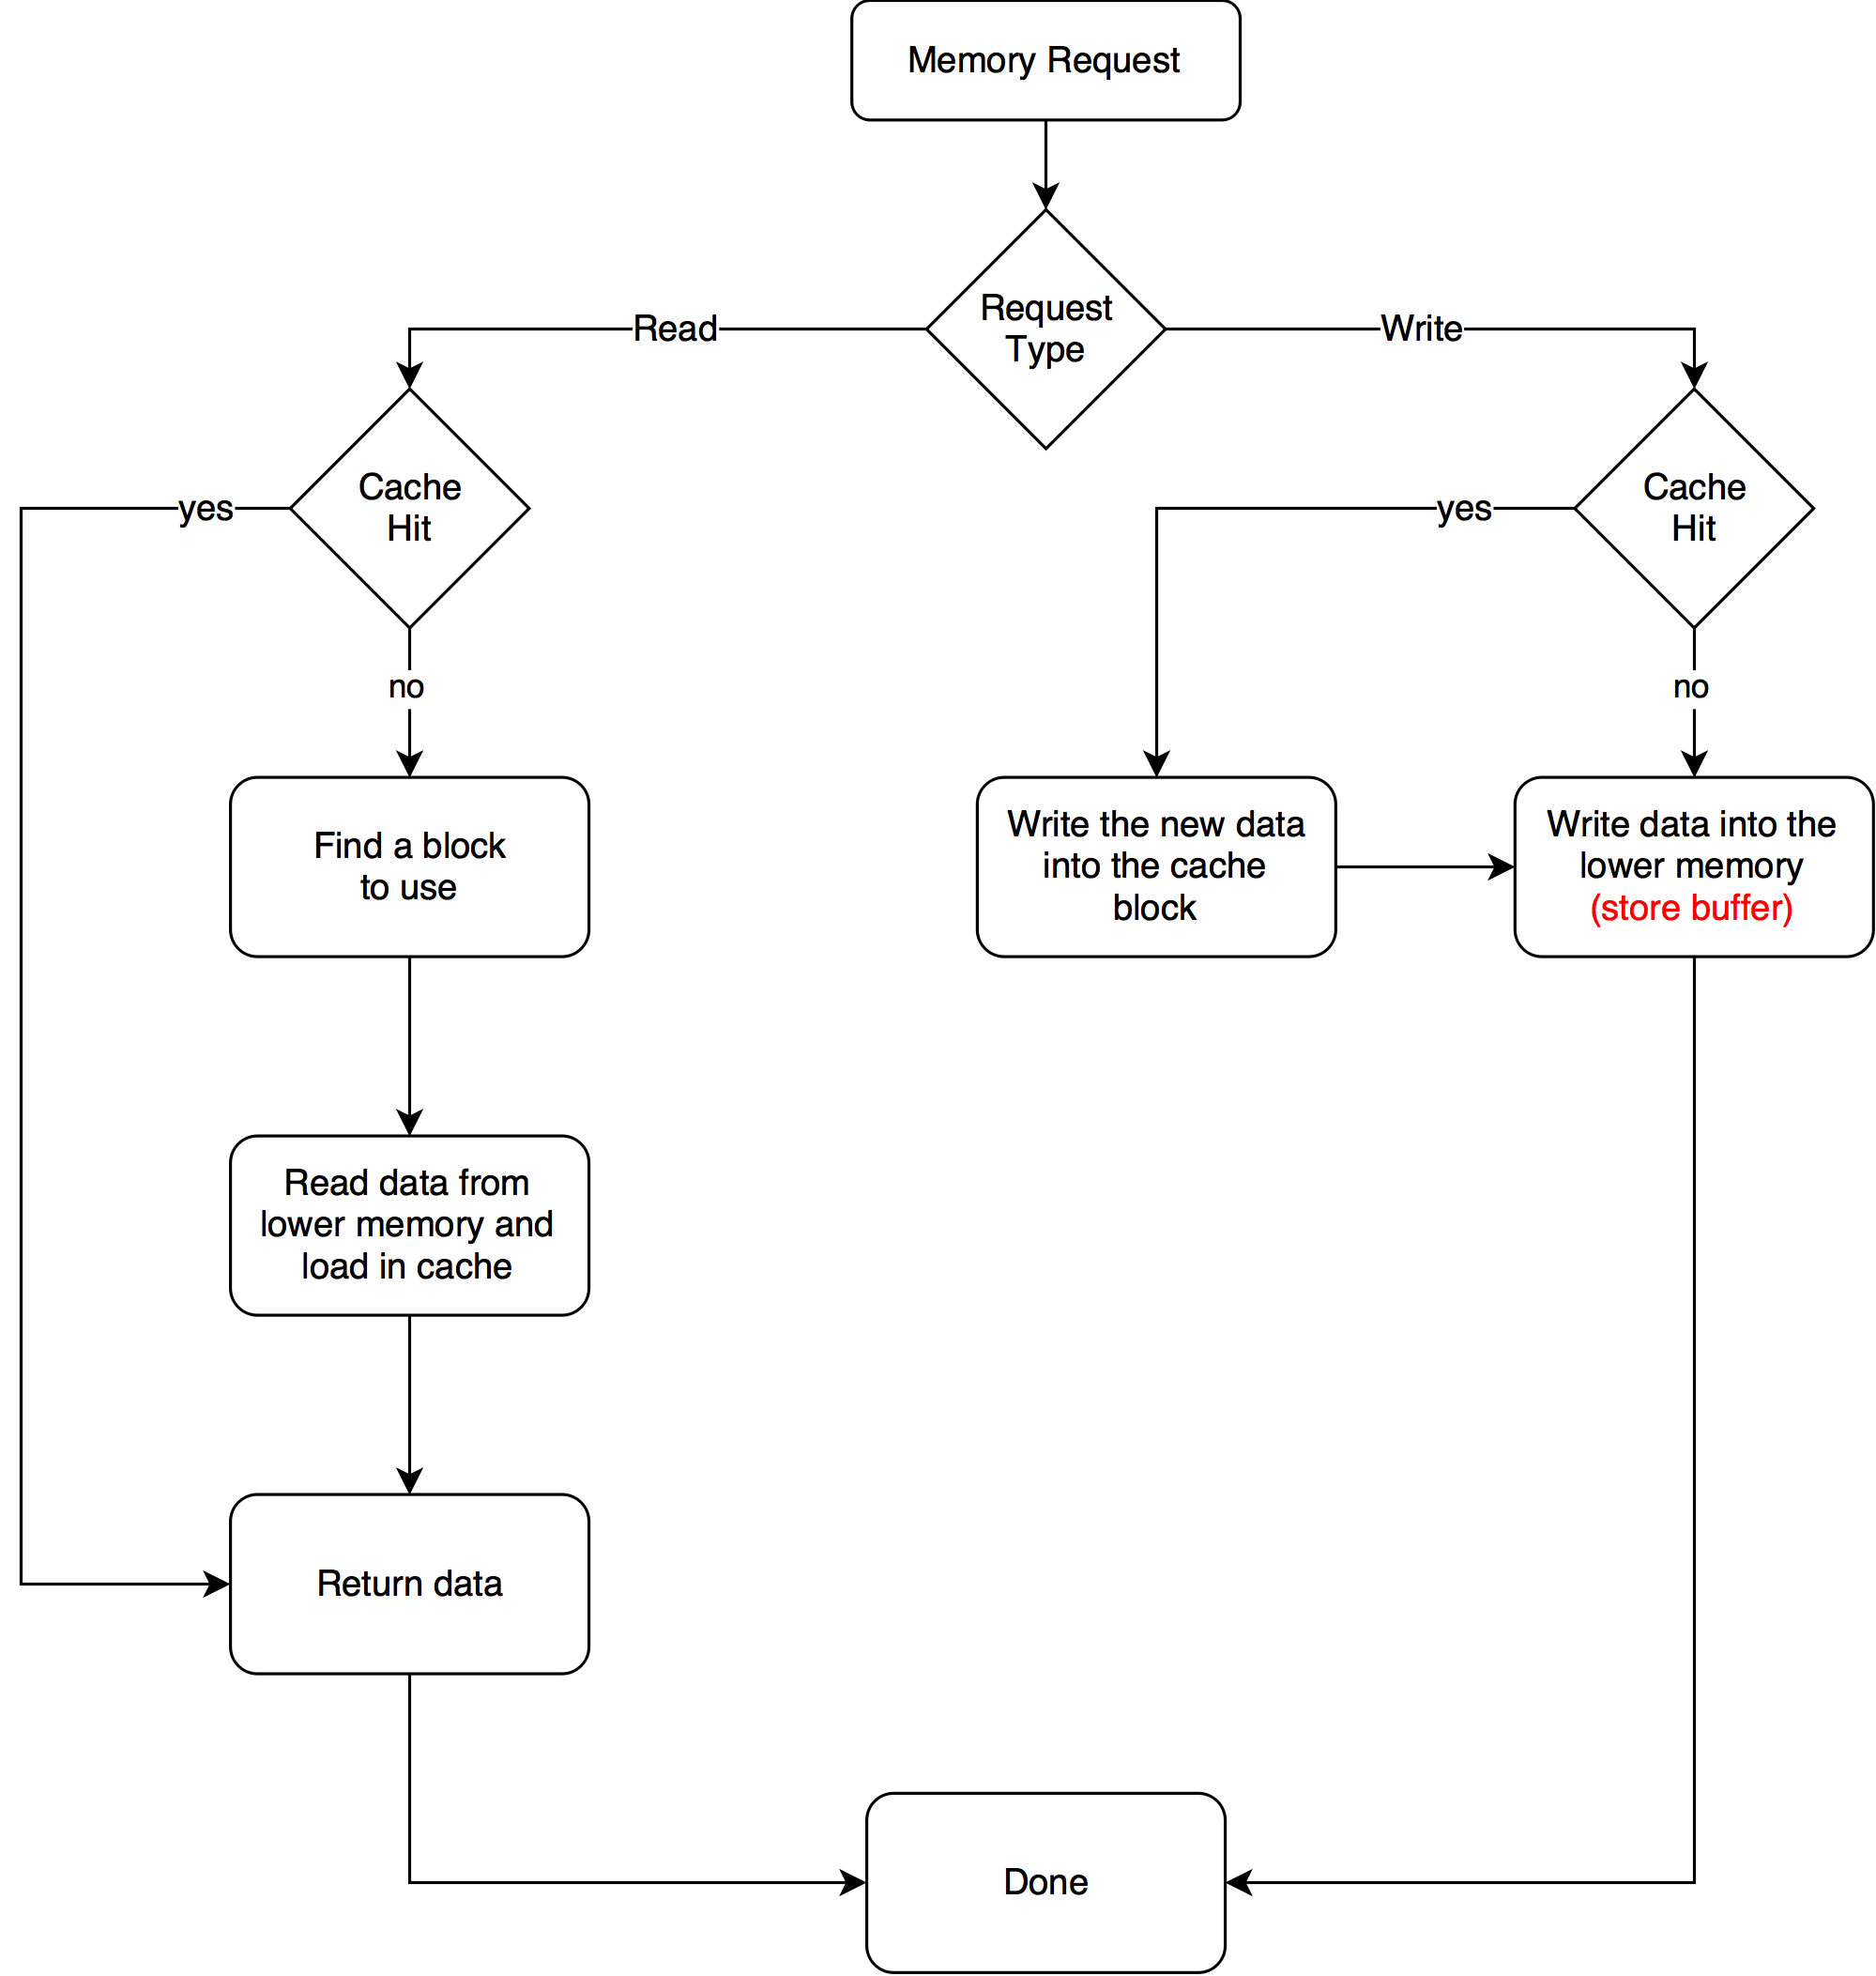
\includegraphics[width=\textwidth]{./pictures/cache_wt_flow.png}
		\caption{Flow diagram showing the original mor1kx \textit{write-through} working principle.}
		\label{wt_flow_diagram}
	\end{center}
\end{figure}

\section{System Configurations}
Different system configurations can be achieved by enabling and disabling the data cache and/or the store buffer. Both the modules are generated in the scope of the LSU module.

\begin{table}[H]
	\begin{center}
		\begin{tabular}{c | c | c}
			\hline
			Config. & Data Cache & Store Buffer \\
			\hline
			\hline
		    1 & Enabled & Enabled \\
		    \hline
		    2 & Enabled & None \\
		    \hline
		    3 & None & Enabled \\
		    \hline
		    4 & None & None \\
			\hline
		\end{tabular}
	\end{center}
	\caption{Potential system configurations of the original mor1kx implementation. The data cache and the store buffer are generated within the LSU \textit{Cappuccino} module.}
	\label{wt-system-configurations}
\end{table}